\section{Test Allocation Mechanism}\label{chapter.allocation_mechanism}
\thispagestyle{plain}

Since the test type intended for \toolname \space generally runs slowly, designing a mechanism that would efficiently allocate tests to test machines in an attempt to minimize the duration it takes to find and execute the schedule. This mechanism has been named OptiX, and will be thoroughly described in the following section. As explained in Chapter \ref{chapter.background}, an alternative allocation mechanism has also been implemented using Google's OR-tools library, and has been used establish a benchmark for use in the evaluation process of OptiX, which will be presented in the next chapter. The alternative allocation mechanism has been named \emph{ORX}, and implementation details will be explained subsequently. \improvement{TODO: CHANGE THIS! Include algorithm listing of OptiX}

\subsection{OptiX}\label{subsection.optix}

\improvement{TODO: Say something about the initial allocation of OptiX using a LJF approach.}

The OptiX allocation mechanism consists of a sequence three steps; sorting, initial allocation and enhancement iterations. It can be seen as an extended greedy algorithm, and will be explained in this section.

In order to give a better understanding of how the algorithm works, a demonstration example will be used throughout the explanation. In this example, we assume that there are three test machines connected to the system, as well as the test set listed in Table \ref{testsuite}. Note that the durations of the tests intended for \toolname \space generally range between approximately 30 and 120 seconds, but this example deliberately uses shorter durations to better illustrate how the mechanism works.

\begin{table}[h!]
  \begin{tabular}{c c c}
    \hline
    \textbf{Test} & \textbf{Duration} & \textbf{Executable on}\\
    \hline
    $t_{1}$     &   6   &   $m_{1}$, $m_{2}$, $m_{3}$\\
    $t_{2}$     &   3   &   $m_{1}$, $m_{2}$, $m_{3}$\\
    $t_{3}$     &   8   &   $m_{1}$, $m_{2}$, $m_{3}$\\
    $t_{4}$     &   5   &   $m_{1}$, $m_{2}$, $m_{3}$\\
    $t_{5}$     &   3   &   $m_{1}$, $m_{2}$, $m_{3}$\\
    $t_{6}$     &   4   &   $m_{1}$, $m_{2}$, $m_{3}$\\
    $t_{7}$     &   7   &   $m_{1}$\\
    $t_{8}$     &   3   &   $m_{2}$\\
    $t_{9}$     &   9   &   $m_{3}$\\
    $t_{10}$    &   5   &   $m_{1}$, $m_{3}$\\
    \hline
  \end{tabular}
  \centering
  \caption{Example Test Set}
  \label{testsuite}
\end{table}

\comment{(extended) greedy algorithm with iterations.}

%\vspace{7px}
\noindent \textbf{\betterfakesc{Sorting}}\\
\noindent The first step is a preparation for the initial allocation. In a scenario where toward the end of the allocation, all tests waiting to be allocated could only be executed on one specific machine, the overall execution time could be greatly affected. Similarly, if toward the end of the initial allocation the last test to be allocated is estimated to have a  This step seeks to avoid such scenarios by strategically ordering the tests before the initial allocation starts. The sorting does not play a crucial role in the allocation mechanism, but it creates an excellent starting point as the tests are sorted in a way that makes them well suited for the initial allocation in the next step.

There are two criteria to the sorting process: the first criteria is the number of machines each test can be executed on, in ascending order, and the second criteria is estimated test duration in descending order.

The test set is first divided into subsets determined by the number of machines they can be executed on. Each of the subsets is then sorted by their estimated duration in descending order, so that the longest tests are placed first and the shortest are placed last. The list is then assembled again.

\begin{figure}[ptb]
    \centering
    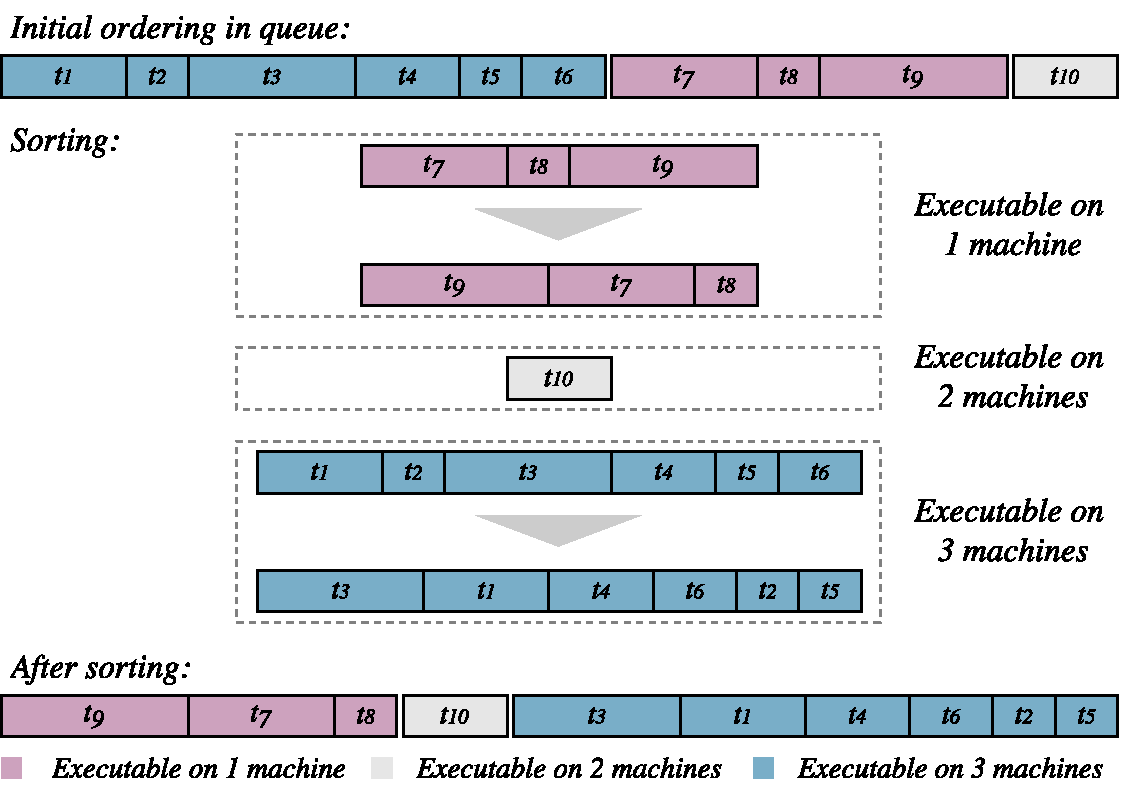
\includegraphics[width=\textwidth]{figures/new/sorting.pdf}
    \thisfloatpagestyle{plain}
    \caption{Sorting of Example Test Set}
    \label{fig.sorted_test_suite}
\end{figure}

Figure \ref{fig.sorted_test_suite} illustrates how the sorting method works with the example test set introduced earlier. Since $t_{7}$, $t_{8}$ and $t_{9}$ can only be executed on a single machine each, these are placed first in descending order of their duration. Test $t_{10}$, which can be executed on two machines, comes thereafter. Finally, tests $t_{1}$ through $t_{6}$, which can run on all of the machines, are ordered and added to the list of tests.






\vspace{7px}
\noindent \textbf{\betterfakesc{Initial Allocation}}\\
\noindent The initial allocation is a greedy algorithm, which means that it always makes a locally optimal choice in the hopes that it will give the best result in the end \cite{Algorithms}. Greedy algorithms are powerful and work well for an extensive spectrum of problems. Creating a greedy algorithm was a suitable choice for this problem.

This step creates the foundation of the test allocations. After being sorted, the list of tests is looped through, and the tests are allocated one by one, starting with the \emph{longest} of the tests that are executable on the \emph{fewest} machines. Each test is initially allocated to the machine that currently has the shortest overall duration among the machines that the test is executable on.

\begin{figure}[h]
    \centering
    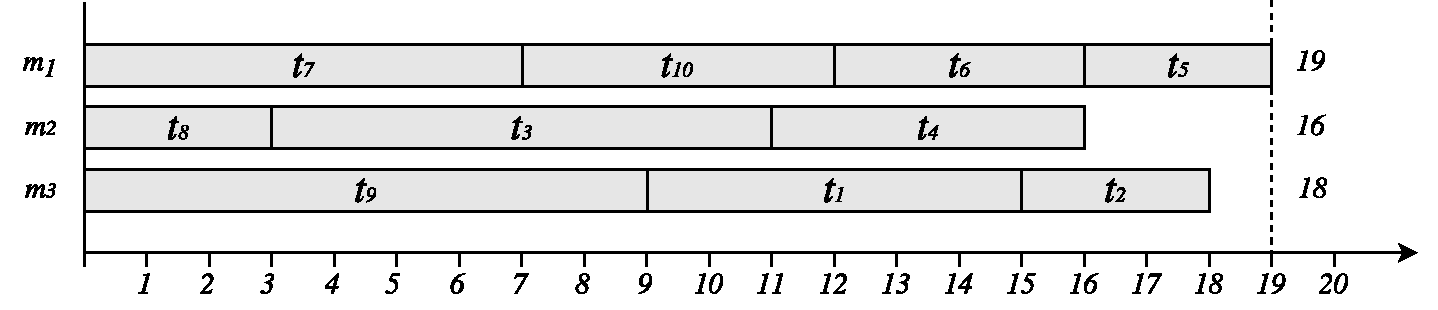
\includegraphics[width=\textwidth]{figures/new/initial_allocation3.pdf}
    %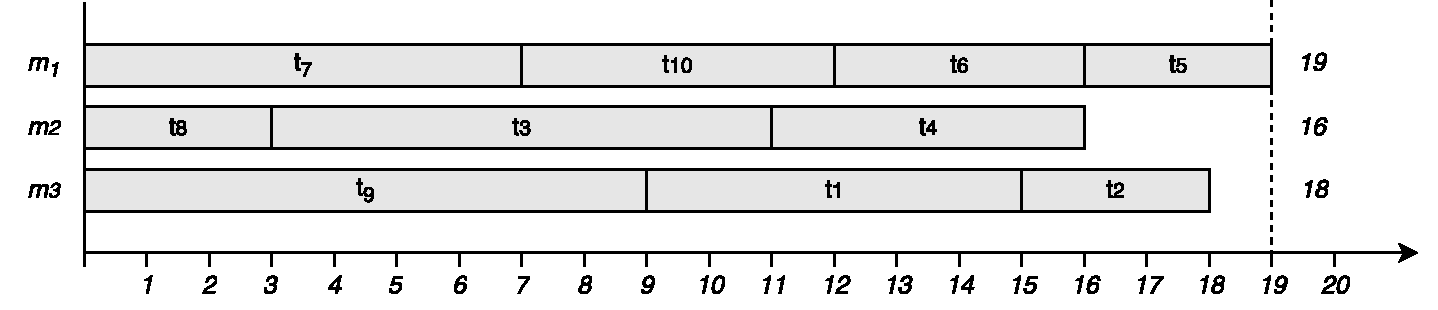
\includegraphics[width=\textwidth]{figures/initial_allocation.pdf}
    \caption{Initial Allocation of Example Test Set}
    \label{fig.initial_allocation}
\end{figure}

Figure \ref{fig.initial_allocation} shows how the test set is initially allocated among the test machines. Tests $t_{9}$, $t_{7}$ and $t_{8}$ are first allocated to $m_{3}$, $m_{1}$ and $m_{2}$ one by one, as each of them can only be executed on that machine. Test $t_{10}$ can be executed on both $m_{3}$ and $m_{1}$, but as the latter currently has the shortest overall execution time, this is the machine it is allocated to. The remaining tests are allocated in the same way. After the initial allocation is finished, the overall execution time is 19. However, the total durations among the machines are slightly uneven, so there might be room for improvement. This will be examined in the last step of OptiX.






\vspace{7px}
\noindent \textbf{\betterfakesc{Enhancement Iterations}}\\
\noindent Greedy algorithms are simple, yet efficient, and provide adequate results most of the time. However, they do not always yield optimal solutions. In order to improve the result, an additional step has been included in the OptiX. This is the most complex element in the process.

The basic idea behind the iteration step is to find subsets of tests among the machine with the longest execution time and the other machines, and swap the two subsets that will result in the largest reduction in overall duration. The subject of each iteration is the machine that currently has the longest execution time. In the case of the example test set, this is $m_{1}$. This will be referred to as the \emph{swapper}. Each of the remaining machines are addressed one by one, starting with $m_{2}$, which is a \emph{swappee} candidate. The tests that are currently allocated to the swapper, but also executable on the swappee candidate are retrieved, which in this case is $t_{5}$ and $t_{6}$. A list of all possible subsets from this set is then created. This is done by using Python's \emph{itertools} library. The same is done the other way around, with $t_{3}$ and $t_{4}$ for the swappee candidate. After this, we examine how each swap would affect the overall duration of the two machines in question. After comparing all subsets, it is concluded that the best swap is $t_{5}$ and $t_{6}$ from $m_{1}$ for $t_{4}$ from $m_{2}$, which will decrease the overall duration among the two machines with 1 second. Since $m_{3}$ can not provide any better options, this swap is conducted. This process will repeat until there is no way to improve the allocations, which in this case is after one swap. Figure \ref{fig.iteration} shows how the subset swap is conducted, and how it affects the overall duration. Although it is not guaranteed to happen, OptiX found an optimal solution to the optimization problem in this example. ORX also found a solution that provided 18 seconds, even though the exact allocations differed slightly.

Upon evaluating each swappee candidate, a naive best-case duration is calculated by adding the durations of all the tests from the two machines and dividing the sum by two. If the time used to search for the best swap exceeds the difference between the total duration of the swapper (here: 19), and this best scenario duration (here: $\frac{19+17}{2} = 18$), which in this case is $1$, we will continue to the next swappee candidate. This means that we will examine the subsets of $m_{2}$ for at most 1 second.

%In an attempt to save time, the subsets are sorted according to their total durations; the swapper subsets descending and the swappee subsets ascending. This ensures that the subsets with the longest total durations are attempted removed from the swapper first.

\begin{figure}[t]
    \centering
    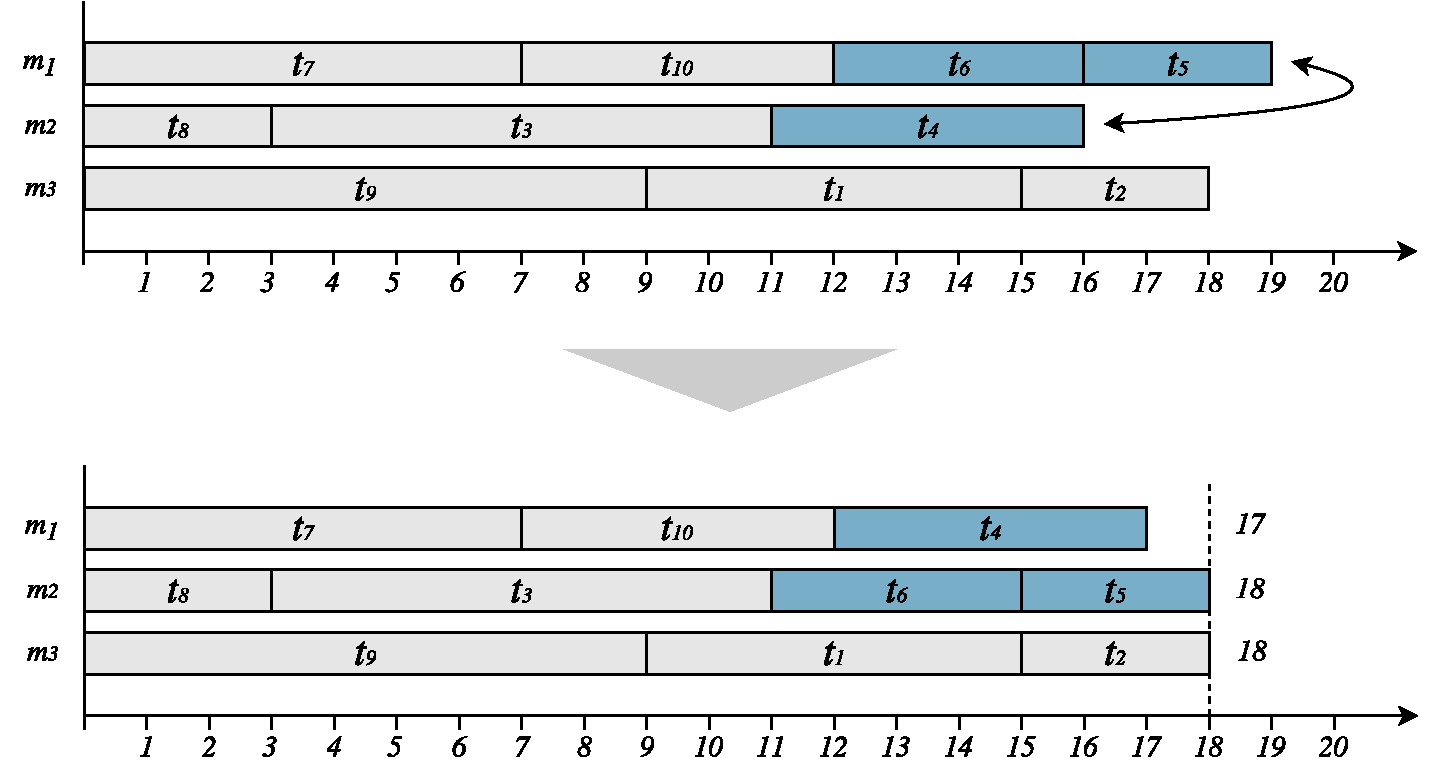
\includegraphics[width=\textwidth]{figures/new/iteration3.pdf}
    %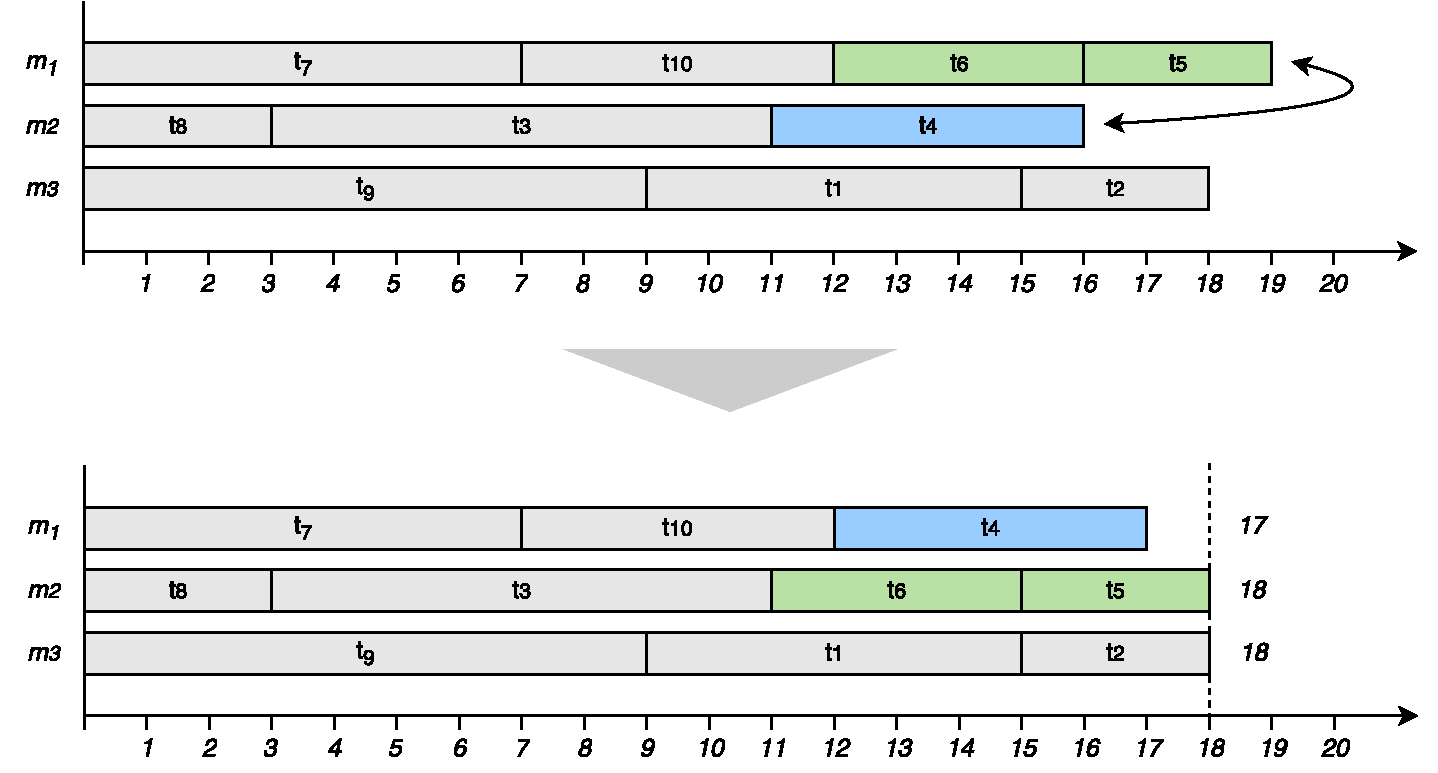
\includegraphics[width=\textwidth]{figures/iterations2.pdf}
    \caption{Enhancement Iteration of Example Test Set}
    \label{fig.iteration}
\end{figure}

Sometimes, however, we want to stop the searching earlier, as continuing is no longer beneficial. For that reason, two stop criteria are introduced:

\begin{enumerate}
    \item Prior to the first enhancement iteration, a naive best-case overall duration value is calculated by dividing the sum of all test durations by the number of machines available. Once the time difference between this value and the maximum machine duration is exceeded, the iteration process will stop.
    \item There is a timeout set to 30 seconds. If the iterations still are not finished at this point, the method will be terminated, and the allocations found up to that point will be kept.
\end{enumerate}

During the development phase, a clear problem stood out; creation of subset lists from extremely large interchangeable test sets between two machines could take several minutes, and sometimes even lead to memory leaks so that the whole system crashed. This was because there was simply too many possible subsets. To work around this problem, a restriction of the maximum size of the subsets had to be established. Through trial and error, the following was decided upon, where $x$ is the maximum size of each subset:

\[
\hfill
    f(x)=\left\{
        \begin{array}{l l}
          x         &   \hspace{20px} \text{if} \hspace{32px} x < 10\\
          20-x      &   \hspace{20px} \text{if} \ 10 \leq x < 20 \\
          1         &   \hspace{20px} \text{if} \ 20 \leq x
        \end{array}
    \right.
\hfill
\]

Thus, if the number of interchangeable tests are 19 or more, the subset list will only consist of single tests in addition to the empty set. Although not optimal, this was a compromise that helped resolve the problem effectively. This means that for large interchangeable sets, tests can only be swapped one against one or moved from one machine to another. It is therefore reasonable to think that better swaps might exist, although identifying these would take too much time and potentially lead to memory leaks. \comment{  Figure \ref{fig.subsets} shows a plot of $f(x)$.

\begin{figure}[h]
    \centering
    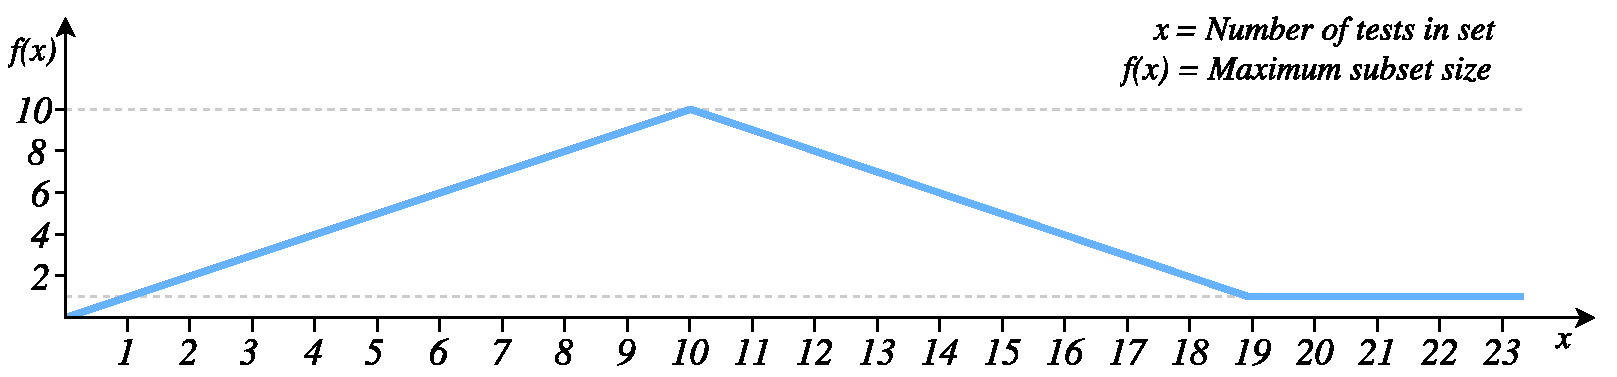
\includegraphics[width=\textwidth]{figures/new/subset_sizes.pdf}
    %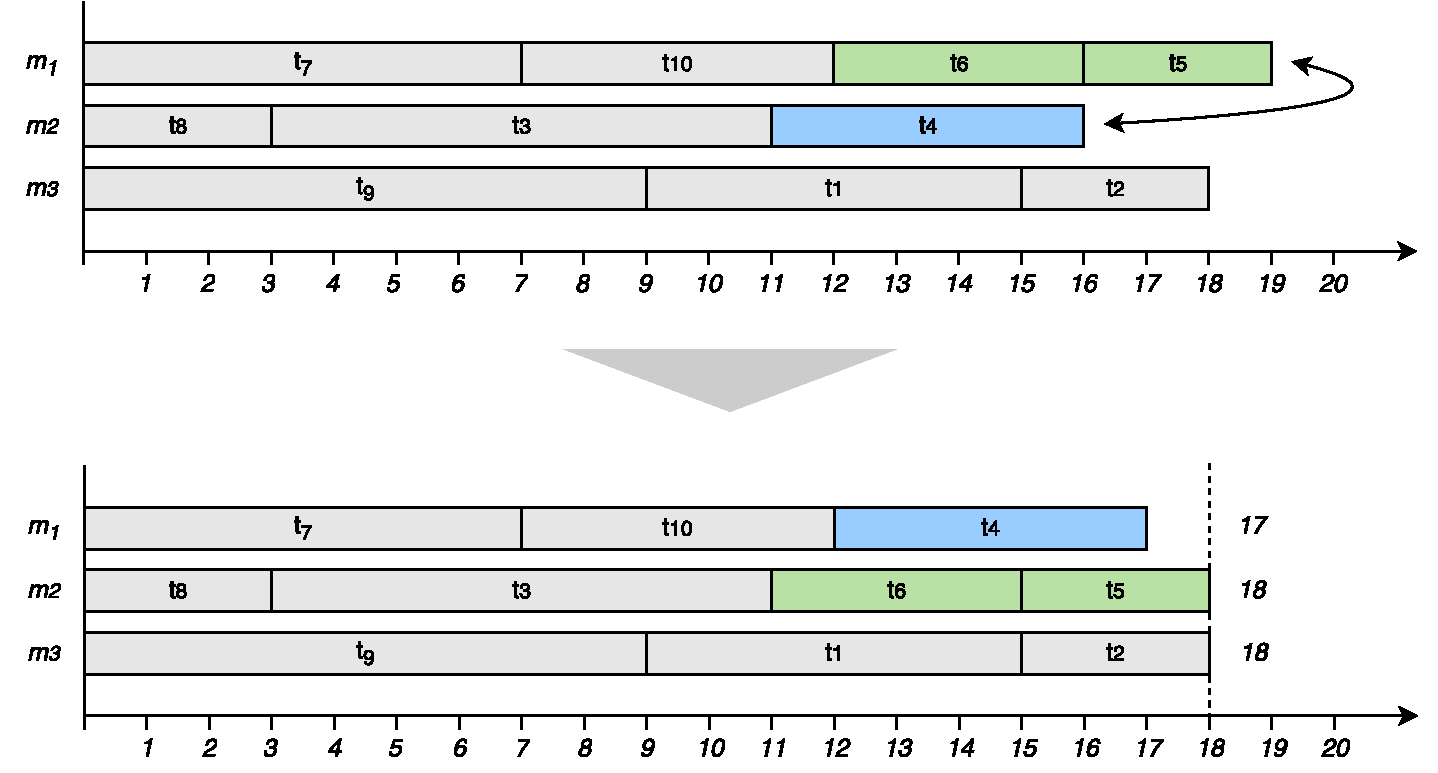
\includegraphics[width=\textwidth]{figures/iterations2.pdf}
    \caption{Maximum Subset Sizes}
    \label{fig.subsets}
\end{figure}
}

Because of the stop criteria described earlier and the subset size restriction, \toolname \space cannot \emph{guarantee} to find an optimal solution to the allocation problem. However, as explained in Section \ref{subsection.cp}, the objective of the optimization problem is to minimize the total time, which means that the time used to search for the best solution is also of high importance, and should be prioritized as such.

\subsection{ORX}

The implementation of ORX is of the same style as the OR-tools example shown in \lstlistingname \space \ref{listing.or_tools} in Chapter \ref{chapter.technology}, but more complex. ORX takes two lists; one containing the durations of the tests, and another containing which machines each test is executable on. OR-tools does not support decimal values, so as opposed to OptiX, ORX regards all test durations as integer values. The \emph{executable on} list is nested, with one list belonging to each test. These inner lists contain binary values representing whether or not the test can be executed on a given machine. It is then added as a constraint that each test should be allocated to exactly one machine, and as the objective that the overall duration should be minimized.

However, there was one major issue upon the implementation of ORX. It was not possible to interrupt or time out the \emph{NextSolution} method. For very small data sets, this was not a problem, but once the data sets grew slightly bigger and the combination of possibilities grew rapidly, the method could take hours. This meant that a set of stop criteria had to be introduced. However, the problem could still not be solved by running the solver in a separate thread, as there is no integrated method of terminating regular threads in Python to the best of the author's knowledge. The problem was solved by introducing Python's \emph{multiprocessing} library.

The solving method is started as a \emph{Process} from the multiprocessing library. In order to allow two processes to share lists, a \emph{Manager} is needed, and to ensure synchronization, a \emph{Lock} has been used. \lstlistingname \space \ref{listing.orx_multiprocess} shows how these multiprocessing modules are used in ORX.

ORX will be terminated if one of the following stop criteria are met:

\begin{itemize}
    \item The search for an improvement has taken 100 times as long as it took to find the previous improvement.
    \item The previous improvement took 10 times as long to find than the improvement itself.
    \item 30 seconds have passed (timeout).
\end{itemize}

\vspace{4mm}
\noindent\begin{minipage}{\textwidth}
\begin{lstlisting}[caption=ORX Multiprocessing, label={listing.orx_multiprocess}]
from multiprocessing import Process, Manager, Lock

manager       = Manager()
allocations   = manager.dict()
max_durations = manager.list()
last_updated  = manager.list()
lock          = Lock()

# ...

p = Process(target=find_solution, args=(durations, executable_on, allocations, max_durations, last_updated, lock))
p.start()

while p.is_alive():
  if lock.acquire():
    if <stop criteria fulfilled>:
      p.terminate()
      break
    lock.release()

# ...

def solution_loop(self, durations, executable_on, shared_allocations, max_durations, last_updated, lock):
    # ...
    
    while solver.NextSolution():
      lock.acquire()
      # ...
      lock.release()
\end{lstlisting}
\end{minipage}
